\documentclass[10pt]{article}
\usepackage[margin=1in, paperwidth=8.5in, paperheight=11in]{geometry}
\usepackage{ifpdf,amsmath, amssymb, comment, color, graphicx, stmaryrd,setspace,enumitem,tikz, fancyhdr, wrapfig, textcomp, units, mathptmx, pdfpages, cancel, multicol, siunitx}
\usepackage{hyperref}
\hypersetup{
    colorlinks=true,
    urlcolor=blue,
}

\setlength{\headheight}{14.5pt}
\newcommand{\Q}{\mathbb{Q}}
\newcommand{\R}{\mathbb{R}}
\newcommand{\Z}{\mathbb{Z}}
\newcommand{\vu}{\mathbf{u}}
\newcommand{\vv}{\mathbf{v}}
\newcommand{\vw}{\mathbf{w}}
\newcommand{\vi}{\mathbf{i}}
\newcommand{\vj}{\mathbf{j}}
\newcommand{\vk}{\mathbf{k}}
\newcommand{\vn}{\mathbf{n}}
\newcommand{\vr}{\mathbf{r}}
\newcommand{\va}{\mathbf{a}}
\newcommand{\vF}{\mathbf{F}}
\newcommand{\vL}{\mathbf{L}}
\newcommand{\vT}{\mathbf{T}}
\newcommand{\vN}{\mathbf{N}}
\newcommand{\proj}{\operatorname{proj}}
\newcommand{\orth}{\operatorname{orth}}
\newcommand\del\nabla
\newcommand\dotp[1][.5]{\,\mathbin{\vcenter{\hbox{\scalebox{#1}{$\bullet$}}}}\,}

% Solution text is in red. If you want the solutions to show, remove the \iffalse from the definition of the \red command.
%\newcommand{\red}[1]{ %\iffalse
%	\textcolor{red}{#1} }%\fi}

\newenvironment{red}{\color{red}}{\ignorespacesafterend}
\newcommand{\blue}[1]{\textcolor{blue}{#1}}
\newcommand{\green}[1]{\textcolor{green}{#1}}
\renewcommand{\section}[1]{\begin{center} \textbf{#1} \\\end{center}}
%
\hyphenpenalty=5000
\setlength{\parindent}{0in}
%\oddsidemargin=-.25in
\allowdisplaybreaks
\pagestyle{fancy}
\renewcommand{\headrulewidth}{0pt}
\lhead{MATH 202}
\rhead{Spring 2023}
%\lfoot{\copyright\ CLEAR Calculus 2010}
\cfoot{}

\begin{document}
%


%\onehalfspacing
\allowdisplaybreaks
%##################################################################
\section{PS\#1: Numerical integration - \red{Answer key} }

\begin{red}
(Note: I split the derivative review questions off into their own separate pdf.)
\end{red}

\textbf{Activity 5.6.3.}

A car traveling along a straight road is braking and its velocity is measured at several different points in time, as given in the following table. Assume that is continuous, always decreasing, and always decreasing at a decreasing rate, as is suggested by the data.

\begin{minipage}{0.3\textwidth}
\[\begin{array}{cc}
\text { seconds, } t & \text { Velocity in } \mathrm{ft} / \mathrm{sec}, v(t) \\
\hline 0 & 100 \\
0.3 & 99 \\
0.6 & 96 \\
0.9 & 90 \\
1.2 & 80 \\
1.5 & 50 \\
1.8 & 0
\end{array}\]
\end{minipage}\qquad
\begin{minipage}{0.7\textwidth}
\hfill
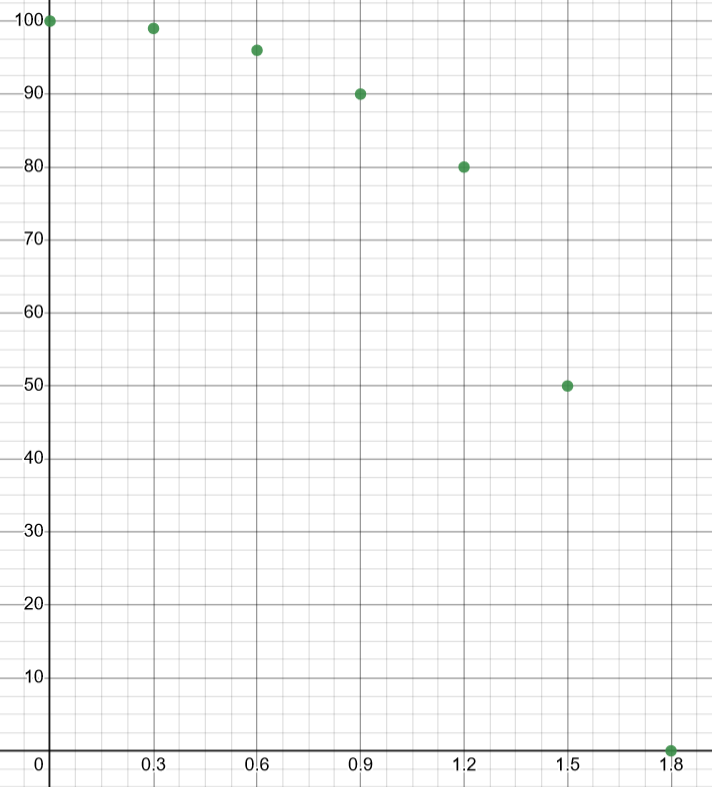
\includegraphics[width=0.5\textwidth]{images/5-6-3-data.png}
\hfill\vphantom{.}
\end{minipage}

\begin{enumerate}[leftmargin=0pt]

\item[b.] What definite integral will give you the exact distance the car traveled on $[0, 1.8]$? \begin{red}
    $\displaystyle\int_{t=0}^{1.8} v(t)\ dt$
\end{red}

\item[c.] Estimate the total distance traveled on $[0, 1.8]$ by computing $L_3$, $R_3$, and $T_3$. Which of these under-estimates the true distance traveled?

\begin{red}
    Note that with 3 rectangles, each rectangle is 0.6 seconds wide. Here are pictures of $L_3$ and $R_3$. Since $v$ is decreasing, $L_3$ is a substantial overestimate and $R_3$ is a substantial underestimate. 

    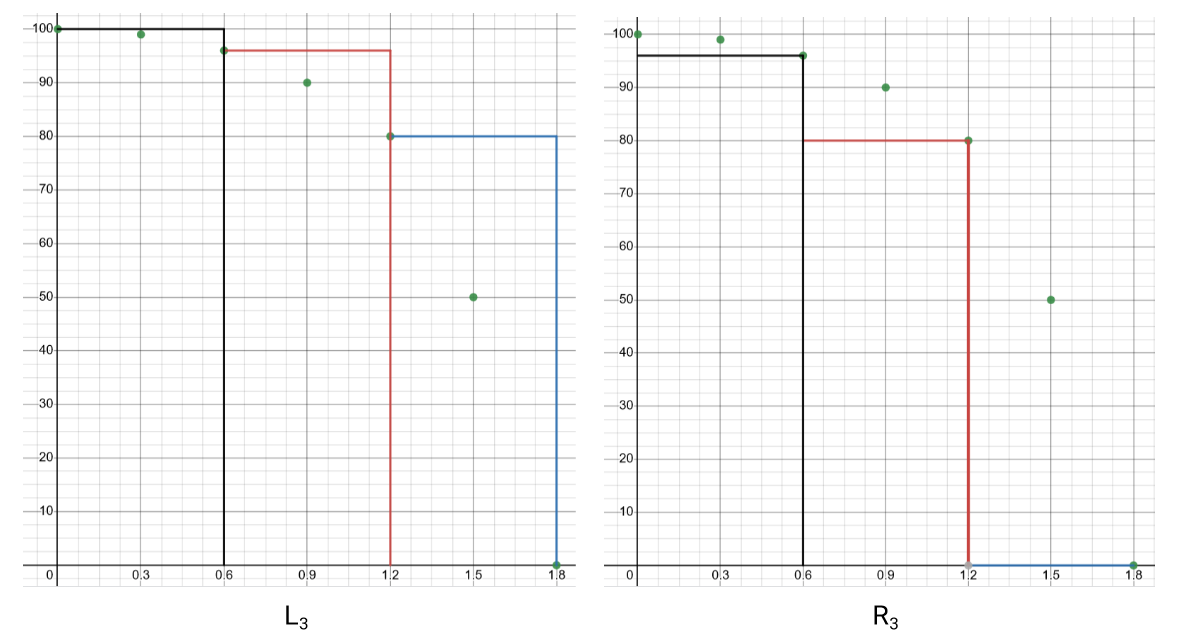
\includegraphics[width=\textwidth]{images/5-6-3-L3-R3.png}

    $L_3 = \SI{100}{ft/s} \cdot \SI{0.6}{s} + \SI{96}{ft/s} \cdot \SI{0.6}{s} + \SI{80}{ft/s} \cdot \SI{0.6}{s} = \SI{165.6}{ft}$. 
    
    $R_3 = \SI{96}{ft/s} \cdot \SI{0.6}{s} + \SI{80}{ft/s} \cdot \SI{0.6}{s} + \SI{0}{ft/s} \cdot \SI{0.6}{s} = \SI{105.6}{ft}$.

    $T_3 = \dfrac{L_3+R_3}{2} = \dfrac{\SI{165.6}{ft}+\SI{105.6}{ft}}{2} = \SI{135.6}{ft}$.
    
    Since $v$ is concave down, the secant lines will lie below $v$, so $T_3$ is also an underestimate. Here's a picture:

    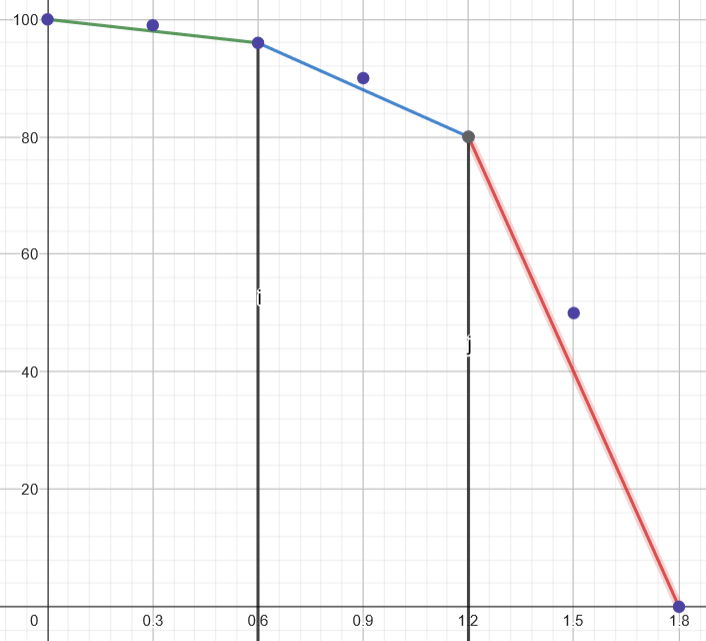
\includegraphics[width=0.7\textwidth]{images/5-6-3-trap.png}
\end{red}

\item[d.] Estimate the total distance traveled on $[0, 1.8]$ by computing $M_3$. Is this an over- or under-estimate? Why?

\begin{red}
    $M_3 = \SI{99}{ft/s} \cdot \SI{0.6}{s} + \SI{90}{ft/s} \cdot \SI{0.6}{s} + \SI{50}{ft/s} \cdot \SI{0.6}{s} = \SI{143.4}{ft}$.

    Remember that midpoint rectangles are the same as tangent trapezoids. Since $v$ is concave down, the tangents are a little above $v$, so this is an overestimate.

    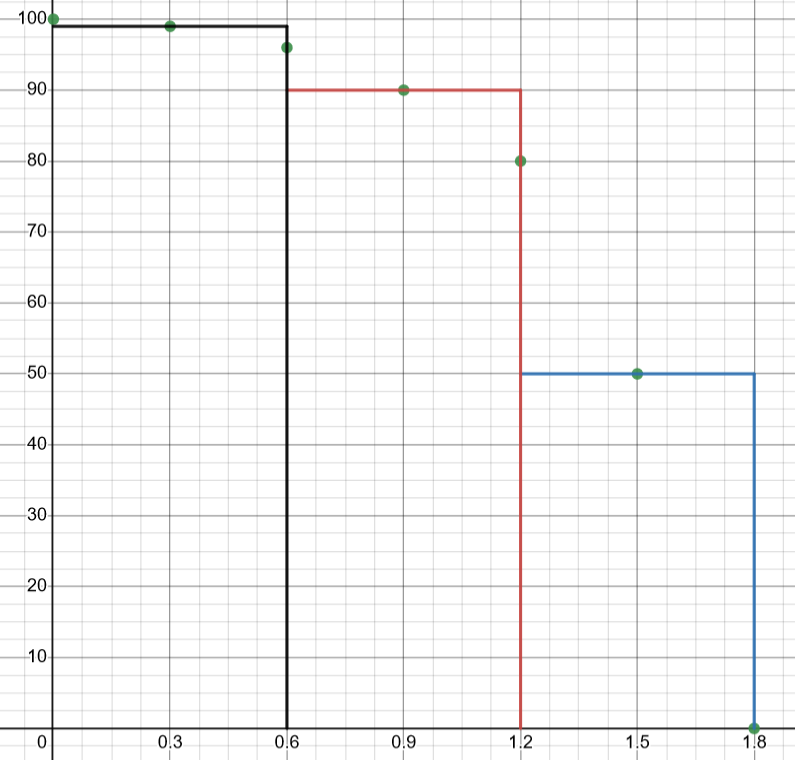
\includegraphics[width=0.55\textwidth]{images/5-6-3-mid.png}
\end{red}

\item[e.] Using your results from (c) and (d), improve your estimate further by using Simpson's Rule.

\begin{red}
    (I'll stick with the convention in the text that this will be called $S_6$ because it uses 6 points. The other convention would be to call this $S_3$ because it uses 3 rectangles.)

    $S_6 = \dfrac{2 M_3 + T_3}{3} = \dfrac{2\cdot\SI{143.4}{ft} + \SI{135.6}{ft}}{3} = \dfrac{\SI{422.4}{ft}}{3} = \SI{140.8}{ft}$.

    Btw, \href{https://www.geogebra.org/calculator/epsungqr}{here's a Geogebra calculator} that shows the parabola-topped rectangles that are the other way to think of Simpson's rule.
\end{red}

\item[f.] What is your best estimate of the average velocity of the car on $[0, 1.8]$? Why? What are the units on this quantity?

\begin{red}
    As best we can estimate, the car traveled $\SI{140.8}{ft}$ in $\SI{1.8}{s}$. 
    
    Therefore, our best guess of average velocity is $\dfrac{\SI{140.8}{ft}}{\SI{1.8}{s}} \approx \SI{78.22}{ft/s}$.
\end{red}

\end{enumerate}
\end{document}